% =================== Deg-Diam problem =================== %
\begin{frame}[t]{Moore Bound: the Degree-diameter Problem}
\begin{itemize}
\item Connect the \textbf{maximum number of routers} ($n$) while keeping \textbf{small length of paths} ($D_{avg}$) and considering that \textbf{the number of router ports is limited} $(\Delta)$.
\item For any $\Delta$-regular graph
$$\displaystyle D\geq \frac{\log(n-1)}{\log(\Delta)}.$$
\item For any node-transitive graph 
$$\displaystyle D_{avg}\geq \frac{nD}{2(n-1)}.$$
\end{itemize}
\end{frame}
% =================== Moore bound =================== %
%\begin{frame}[t]{Moore Bound: Diameter}
%\begin{itemize}
%\item For any $\Delta$-regular graph
% $\displaystyle D\geq \frac{\log(n-1)}{\log(\Delta)}$.
%\end{itemize}
%\begin{table}[h!]
    \begin{tabular}{|c| l |c|}
      \toprule
      \multicolumn{2}{|c|}{\textbf{Topology}}&\multirow{1}{*}{\textbf{$D$}}\\
      \midrule
      \multirow{3}{*}{\textbf{DCN}}&Slimfly & 2\\
      &Jellyfish & 3\\
      &Fat-tree &4\\
      \hline
      \multirow{2}{*}{\textbf{Symmetric}}&Star &\multirow{3}{*}{$O(\log(n))$}\\
      \multirow{2}{*}{\textbf{CG}}&Transposition & \\
      &Hypercube& \\
      \hline
      \multirow{1}{*}{\textbf{Non-symmetric}}&Butterfly&\multirow{1}{*}{$O(\log(n))$}\\
      \multirow{1}{*}{\textbf{CG}}&Bubble-sort& $O(\log(n)^2)$\\
      \bottomrule
    \end{tabular}
  \end{table}
%\end{frame}

% =================== Moore bound =================== %
\begin{frame}[t]{Moore bound: Average Path Distance}
%\begin{itemize}
%\item For any node-transitive graph 
%$\displaystyle D_{avg}\geq \frac{nD}{2(n-1)}$.
%\end{itemize}
\center{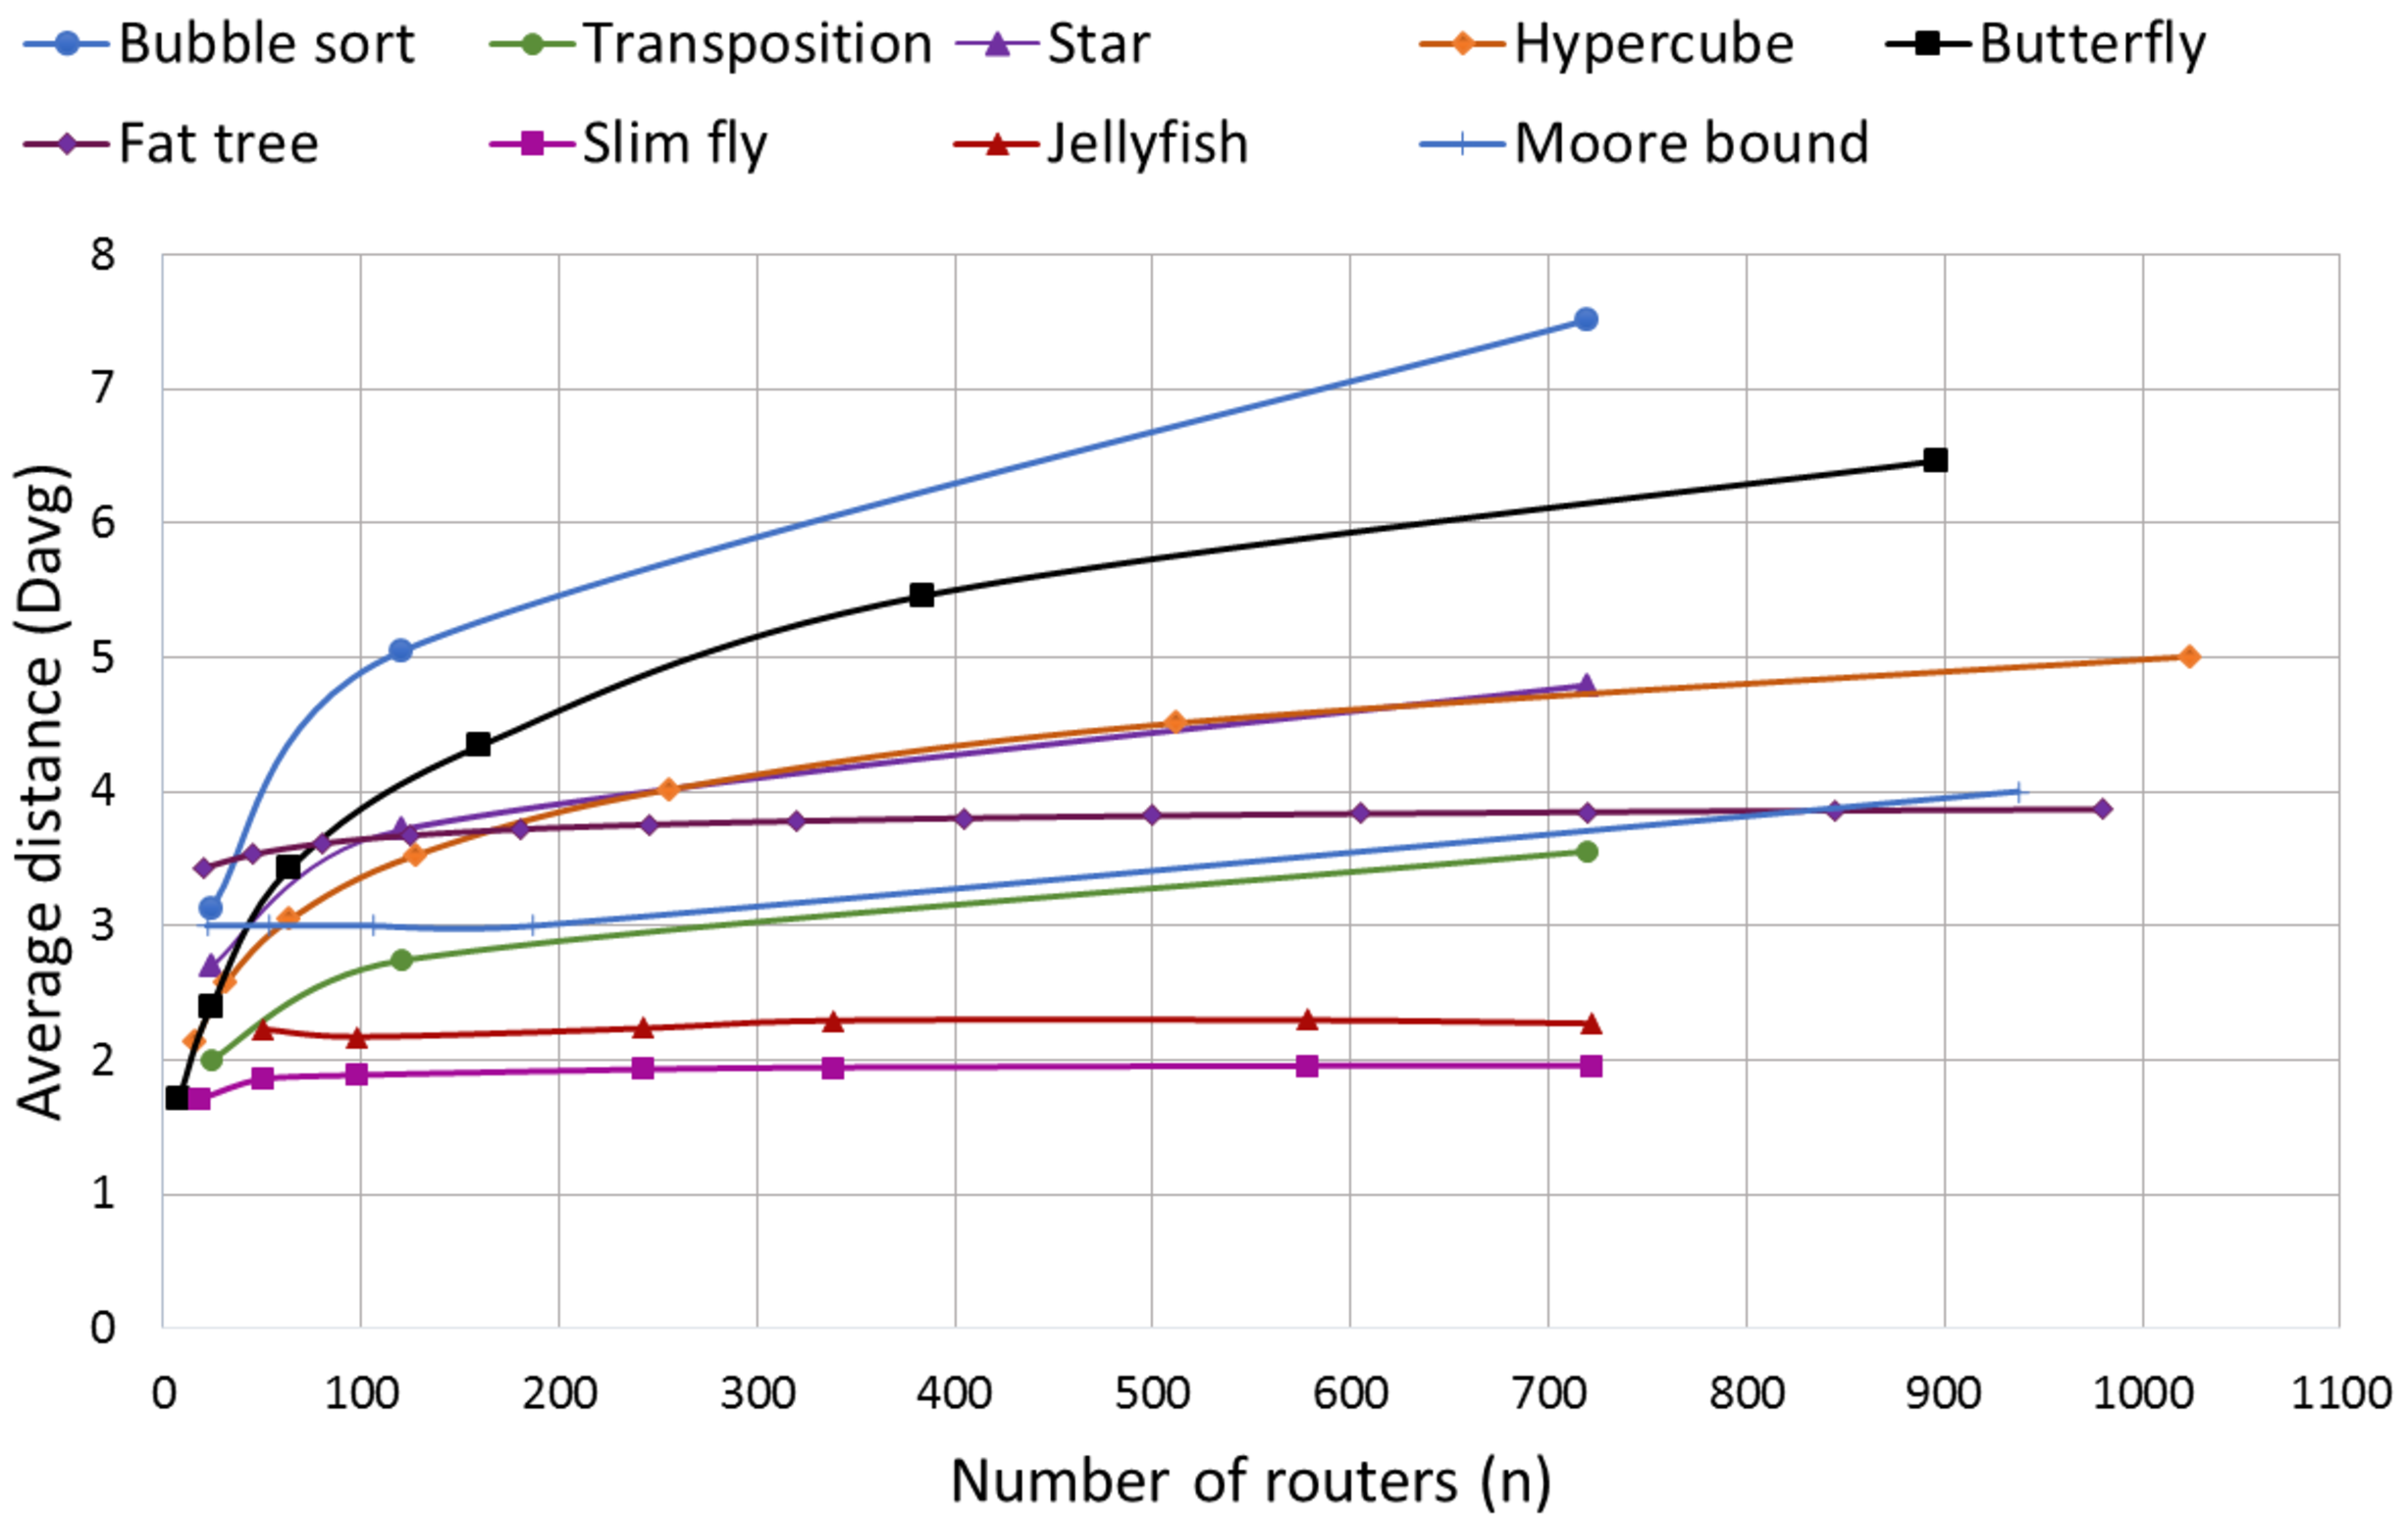
\includegraphics[width=.95\textwidth]{images/avgdist}}
\end{frame}